\documentclass[11pt]{article}

\usepackage[margin=1in]{geometry}
\usepackage{amsmath,amssymb}
\usepackage{enumitem}
\usepackage{framed}
\usepackage{float}
\usepackage{graphicx}
% some definitions
\mathchardef\mhyphen="2D % Define a "math hyphen"
\newcommand{\Gen}{\mathrm{Gen}}
\newcommand{\Enc}{\mathrm{Enc}}
\newcommand{\Dec}{\mathrm{Dec}}
\newcommand{\Prove}{\mathrm{Prove}}
\newcommand{\Vfy}{\mathrm{Vfy}}
\newcommand{\NIZK}{\mathrm{NIZK}}
\newcommand{\secpar}{\lambda}
\newcommand{\pk}{pk}
\newcommand{\sk}{sk}
\newcommand{\ct}{\mathit{ct}}
\newcommand{\foe}{\ensuremath{FO\mhyphen E}}
\newcommand{\nye}{\ensuremath{NY\mhyphen E}}
\newcommand{\size}[1]{\left|#1\right|}
\newcommand{\sampl}{\gets_\$}
\newcommand{\G}{\mathbb{G}}
\newcommand{\Zp}{\mathbb{Z}_p}
\newcommand{\M}{\mathcal{M}}
\renewcommand{\L}{\mathcal{L}}
\newcommand{\geng}{\langle g \rangle}
\renewcommand{\exp}[1]{#1\,\mathrm{exp}}
\newcommand{\cost}[2]{\underbrace{#1}_{\exp{#2}}}
\newenvironment{algsteps}
  {\begin{itemize}[label={},leftmargin=1.5em,topsep=3pt,itemsep=4pt,parsep=0pt]}
  {\end{itemize}}


\setlength{\parindent}{0pt}

\begin{document}

\begin{center}
  {\Large \textbf{Homework Assignment}}\\[0.5em]
  Advanced Encryption Schemes, Fall Semester 2026
\end{center}

\vspace{1em}

\textbf{Name:} {Klevis Imeri}
\hfill
\textbf{Submission deadline:} 29.11.2026, 23:59

\vspace{2em}

\section*{Exercise 1: Naor--Yung transformed ElGamal (mandatory)}
\begin{enumerate}
\item Construction of Naor--Yung transformed ElGamal:

% I removed the tabs in the beggening cause my editor hated them. 

Let's first right definitions that we need (I will just copy definitions from the slides cause its easier to have in one place).
\begin{center}
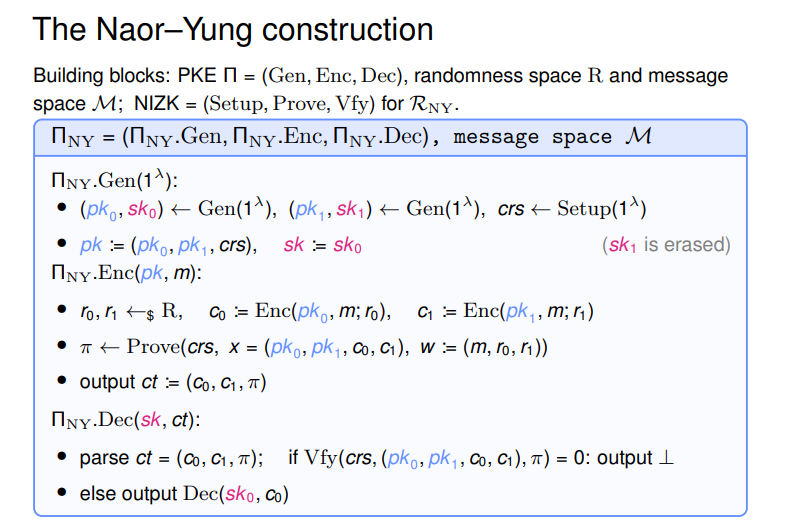
\includegraphics[width=0.80\linewidth]{naor-yung.png}
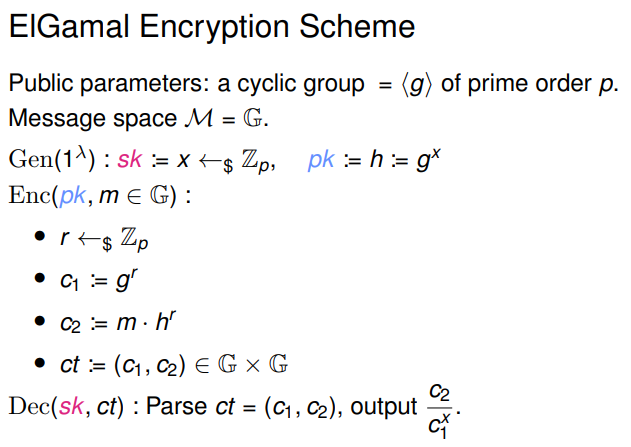
\includegraphics[width=0.70\linewidth]{elgamal.png} 
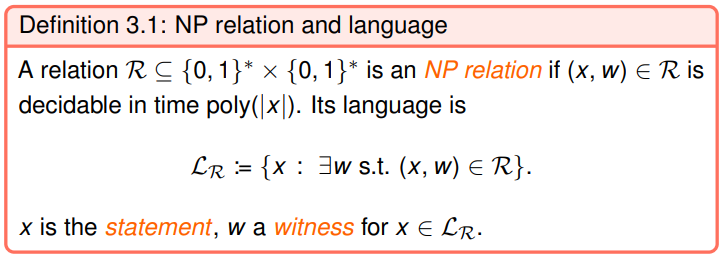
\includegraphics[width=0.75\linewidth]{np-relation-language.png}
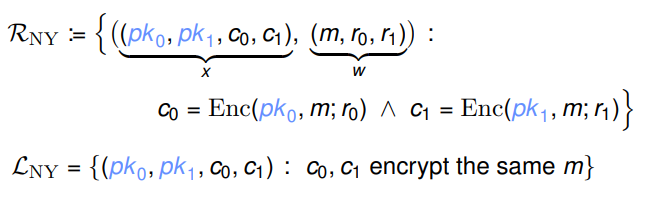
\includegraphics[width=0.75\linewidth]{naor-yung-relation-language.png}
\end{center}
The cyclic group $\G = \geng$ and $\M = \G$ are given from the exercise so the lecture definition of the ElGamal fits.
Below the definition of NP relation and language the format of a generic relatoin and language for a Naor-Yung scheme is given.
Because both encryptions are polynomial the problem is decideble in polynomial time given the witness. 
So the given NY relations fit the def 3.1. 
Everything with subscript E are the functions in the ElGamal scheme. So:

$\Gen_E:$ return $(sk,pk) := (x \sampl \Zp, pk := h:=g^x)$,

$\Enc_E(pk,m \in G; r \sampl \Zp):$ return $ct:=(c_1,c_2) := (g^r, m h^r) \in G \times G$

$\Dec_E(sk = x, ct):$ parse $ct = (c_1,c_2)$; return $\frac{c_2}{c_1^x}$.

Given this information we just have to fill the table below.
\begin{framed}  
  $\L_{\nye} = \{(pk_0,pk_1,c_0,c_1):\exists m\in\M, r_0,r_1 \in \Zp, c_0=\Enc_E(pk_0,m;r_0) \land c_1=\Enc_E(pk_1,m;r_1)\}$

  ${\Gen_{\nye}(1^\secpar)}:$ 
  \begin{algsteps}
    \item ($sk_0$,$pk_0$) $\gets$ $\Gen_E(1^\secpar)$, ($sk_1$,$pk_1$) $\gets$ $\Gen_E(1^\secpar)$
    \item return $(pk,sk):=((pk_0,pk_1),sk_0)$ \hfill ($sk_1$ is erased)
  \end{algsteps}

  $\Enc_{\nye}(\pk, m):$ 
  \begin{algsteps}
    \item $r_0$,$r_1$ $\sampl \Zp$, $c_0 := \Enc_E(pk_0,m;r_0)$, $c_1 := \Enc_E(pk_1,m;r_1)$ \hfill $c_0=(c_{00},c_{01})$
    \item $\pi \gets \Prove(x=(pk_0,pk_1,c_0,c_1), w:=(m,r_0,r_1))$ \hfill $c_1=(c_{10},c_{11})$
    \item return $\ct := (c_0,c_1,\pi)$
  \end{algsteps}

  $\Dec_{\nye}(\sk, \ct):$ 
  \begin{algsteps}
    \item parse $\ct = (c_0,c_1,\pi)$; if parsing fails, return $\bot$.
    \item if $\Vfy((pk_0,pk_1,c_0,c_1),\pi)=0$: return $\bot$; else return $\Dec_E(sk_0,c_0)$.
  \end{algsteps}
\end{framed}
The only thing to note here that we provided the randomness to the encrytion of ElGamal, instead of ElGalal encrytion generating the r themself,
because we needed the the randomness to generate the prove.

\item Comparison table:
\begin{center}
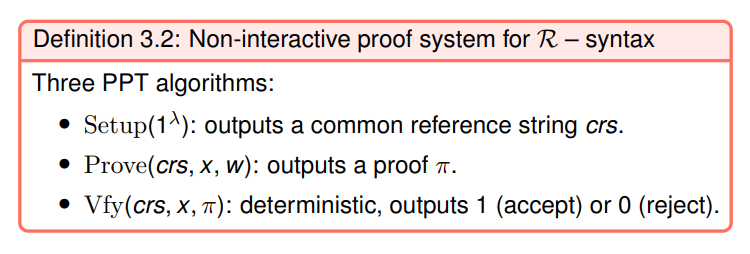
\includegraphics[width=0.75\linewidth]{nizk-syntax.png}
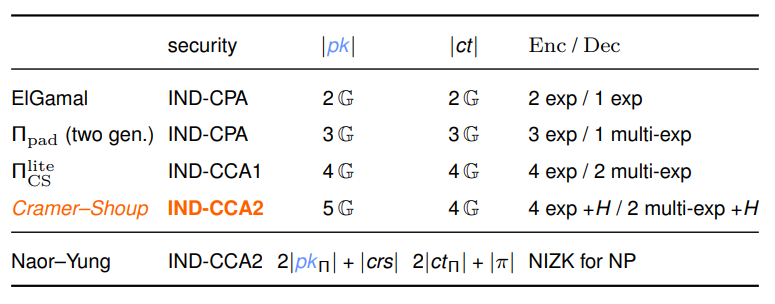
\includegraphics[width=0.75\linewidth]{encryption-cost-reference.png}
\end{center}
The table for with Cramer-Shoup vs Naur-Yung it is just for reference here how the notation is used in lecture, or how something similar was done in the lecture.
From exercise our NIZK is in ROM (and wihtout crs) with prove costing 5 exponenciations and verifying 10, so:

$\Prove^H(x,w):$ return $\pi$ \hfill Cost $\exp{5}$

$\Vfy^H(x,\pi):$ return $b\in \{0,1\}$ \hfill Cost $\exp{10}$

$\Gen_E:$ return $(sk,pk) := (x \sampl \Zp, pk := h:=\cost{g^x}{1})$, \hfill Cost $\exp{1}$

$\Enc_E(pk,m \in G; r \sampl \Zp):$ return $ct:=(c_1,c_2) := (\cost{g^r}{1}, m\cost{h^r}{1}) \in G \times G$ \hfill Cost $\exp{2}$

$\Dec_E(sk = x, ct):$ parse $ct = (c_1,c_2)$; return $\frac{c_2}{\cost{c_1^x}{1}}$. \hfill Cost $\exp{1}$

$\Gen_{\nye}(1^\secpar):$ \hfill Cost $\exp{2}$
\begin{algsteps}
  \item $(sk_0,pk_0) \gets \cost{\Gen_E(1^\secpar)}{1}$, $(sk_1,pk_1) \gets \cost{\Gen_E(1^\secpar)}{1}$
  \item return $(pk,sk):=((pk_0,pk_1),sk_0)$
\end{algsteps}

$\Enc_{\nye}(\pk, m):$ \hfill Cost $\exp{9}$
\begin{algsteps}
  \item $r_0,r_1 \sampl \Zp$, $c_0 := \cost{\Enc_E(pk_0,m;r_0)}{2}$, $c_1 := \cost{\Enc_E(pk_1,m;r_1)}{2}$
  \item $\pi \gets \cost{\Prove(x=(pk_0,pk_1,c_0,c_1), w:=(m,r_0,r_1))}{5}$
  \item return $\ct := (c_0,c_1,\pi)$
\end{algsteps}

$\Dec_{\nye}(\sk, \ct):$ \hfill Cost at most $\exp{11}$
\begin{algsteps}
  \item parse $\ct = (c_0,c_1,\pi)$; if parsing fails, return $\bot$.
  \item if $\cost{\Vfy((pk_0,pk_1,c_0,c_1),\pi)}{10}=0$: return $\bot$; else return $\cost{\Dec_E(sk_0,c_0)}{1}$.
\end{algsteps}

From exercise $\pi = (g_0,...,g_4,s_0,...,s_4)$ s.t $g_i \in \G \; \land s_i \in  \Zp \land$ $\size{g_i} = \size{s_i} = 32\,\text{bytes} = 256\,\text{bits}$ 



pk in NY without crs is just ($pk_0$,$pk_1$) for $pk_0$,$pk_1$ in $\G$.

sk is just $sk_0$ which is just a $sk_0 \sampl \Zp$.

ct is a bit more interesting $\ct = (c_0,c_1,\pi)=((c_{00},c_{01}), (c_{10},c_{11}),(g_0,...,g_4,s_0,...,s_4))$

\begin{table}[H]
  \begin{tabular}{l|c|c}
    & NY-E (mandatory) & FO-E (only for option B)\\ \hline
    
    $\size{\pk}$ (asymptotic)
    & 2$\G$ 
    &  
    \\
    
    $\size{\pk}$ (bits)
    & $2 \cdot 32 \cdot 8=512$ 
    & 
    \\
    
    $\size{\sk}$ (asymptotic)
    & $1\Zp$
    & 
    \\
    
    $\size{\sk}$ (bits)
    & $32 \cdot 8 = 256$ 
    &
    \\
    
    $\size{\ct}$ (asymptotic)
    & $9\G$ $5\Zp$
    & 
    \\
    
    $\size{\ct}$ (bits)
    & $(9+5)\cdot32\cdot8=3584$ 
    &
    \\
    
    \# operations in $\Enc$
    & $\exp {9}$ 
    & 
    \\
    
    \# operations in $\Dec$
    & $\exp {11} (10$ if $\bot)$ 
    & 
    \\
    
    proof assumptions
    & DDH for ElGamal NIZK with (*)  
    &
    \\
    
    model
    & ROM 
    &
    \\
    
    security
    & IND-CCA2 
    & 
  \end{tabular}
  \caption{
    For asymptotic sizes count the number of group elements and scalars.
    For the number of operations count only expensive operations such as exponentiations and oracle calls.
  }
\end{table}
\end{enumerate}

(*) commpleteness, zero-knowledge, one-time simulation soundness. Also worth mentioning that if we just wanted 
IND-CCA1 then NIZK with soundness instead of simulation soundness would be enough.
Also we assune sapling from $\Zp$ is efficient and does not require exponenciation.

\section*{Exercise 2: NIZK optimizations (option A)}
Our goal here is to define a NIZK (here we try in ROM without crs) so:

$\Prove^H(x,w):$ return $\pi$ \hfill Cost $\exp{<5}$

$\Vfy^H(x,\pi):$ return $b\in \{0,1\}$ \hfill Cost $\exp{<10}$

For:

$\L_{\nye} = \{(pk_0,pk_1,c_0,c_1):\exists m\in\M, r_0,r_1 \in \Zp, c_0=\Enc_E(pk_0,m;r_0) \land c_1=\Enc_E(pk_1,m;r_1)\}$

In NY and for INC-CCA2 we need completeness, zero-knowledge, simulation soundness.

In the lecture we had the definitions below for NIZK properties but they are with a crs.

\begin{center}
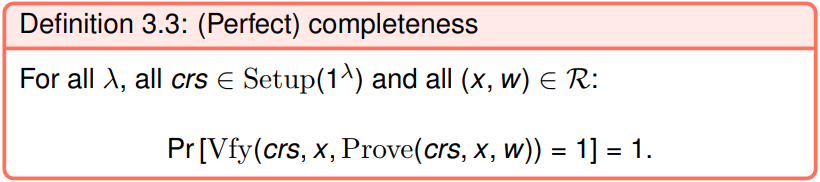
\includegraphics[width=0.75\linewidth]{nizk-completeness.png}
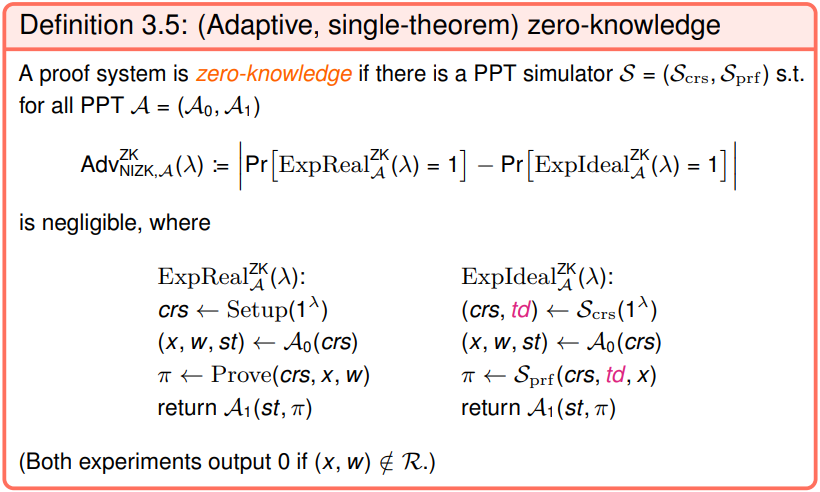
\includegraphics[width=0.75\linewidth]{nizk-zero-knowledge.png}
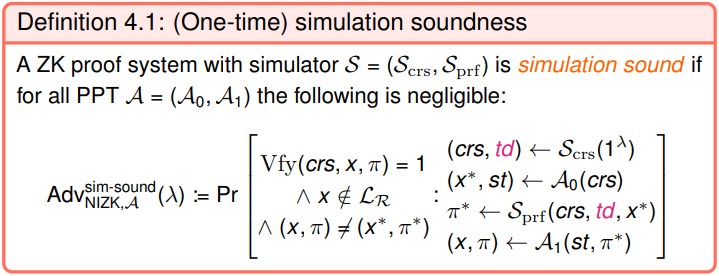
\includegraphics[width=0.75\linewidth]{nizk-simulation-soundness.png}
\end{center}

\begin{minipage}{\linewidth}
Now we give the $\NIZK_{\L_{\nye}}$.

\begin{framed}
$x=(pk_0,pk_1,c_0,c_1)$, $c_0=(c_{00},c_{01})$, $c_1=(c_{10},c_{11})$, $w=(m,r_0,r_1)$.

$H:\{0,1\}^*\to\Zp$ is a random oracle; its inputs use canonical, unambiguous encodings.

$\Prove^H(x,w):$
\begin{algsteps}
  \item $a_0,a_1\sampl\Zp$
  \item $A_0:=g^{a_0}$, $A_1:=g^{a_1}$, $A_2:=\frac{pk_0^{a_0}}{pk_1^{a_1}}$
  \item $e:=H(x,A_0,A_1,A_2)$
  \item $z_0:=a_0+er_0\pmod p$, $z_1:=a_1+er_1\pmod p$
  \item return $\pi:=(A_0,A_1,A_2,z_0,z_1)$
\end{algsteps}

$\Vfy^H(x,\pi):$
\begin{algsteps}
  \item parse $\pi=(A_0,A_1,A_2,z_0,z_1)$; reject malformed inputs or noncanonical encodings.
  \item check that all public-key, ciphertext, and commitment components are in $\G$, and $z_0,z_1\in\Zp$; otherwise return $0$.
  \item $D:=\frac{c_{01}}{c_{11}}$, $e:=H(x,A_0,A_1,A_2)$
  \item return $1$ if all three equations hold; otherwise return $0$:

  $g^{z_0}=A_0c_{00}^{e},\quad g^{z_1}=A_1c_{10}^{e},\quad \frac{pk_0^{z_0}}{pk_1^{z_1}}=A_2D^{e}.$
\end{algsteps}
\end{framed}
\end{minipage}

\section*{Exercise 3: Fujisaki--Okamoto transformed ElGamal variant (option B)}
\begin{enumerate}
\item ...
\item Construction of $\Pi$:
\begin{framed}
  Any helper definitions you might want to define.
  
  \({\Gen(1^\secpar)}:\) ...
  
  \(\Enc(\pk, m):\) ...
  
  \(\Dec(\sk, \ct):\) ...
\end{framed}
... %Explanation of this scheme.

\item Construction of Fujisaki--Okamoto transformed $\Pi$:
\begin{framed}
  Any helper definitions you might want to define.
  
  \({\Gen_{\foe}(1^\secpar)}:\) ...
  
  \(\Enc_{\foe}(\pk, m):\) ...
  
  \(\Dec_{\foe}(\sk, \ct):\) ...
\end{framed}
\item %Don't forget to fill the FO-E column of the table in exercise 1. 
Comparison results: ...
\end{enumerate}



\end{document}
